\chapter{Results}

\label{cha:results}

In this chapter, we first evaluate the neural network against various agents to validate that it has learned how to play the game. Secondly, we describe each concept we intend to examine the neural network against. Thirdly, we take a look at the changes in the emphasis of the neural network during training. The main point of interest there being whether the neural network notices simple HLCs early then stops considering them as the network improves.

\section{Evolution of the Neural Networks Win Rate}

\begin{figure}
    \begin{small}
        \begin{center}
            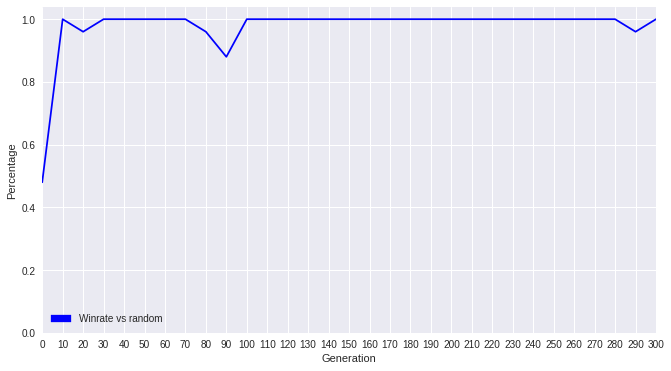
\includegraphics[width=0.7\textwidth]{graphics/winratevsrandom.png}
        \end{center}
        \caption{Winrate vs random agent}
        \label{fig:winratevsrandom}
    \end{small}
\end{figure}

\begin{figure}
    \begin{small}
        \begin{center}
            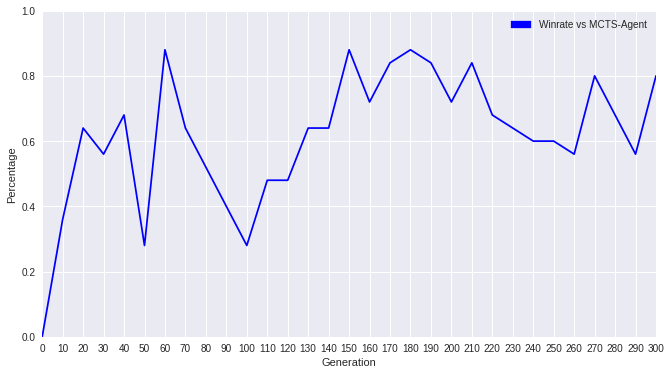
\includegraphics[width=0.7\textwidth]{graphics/winratevsmcts.png}
        \end{center}
        \caption{Winrate vs MCTS agent}
        \label{fig:winratevsmcts}
    \end{small}
\end{figure}

\begin{figure}
    \begin{small}
        \begin{center}
            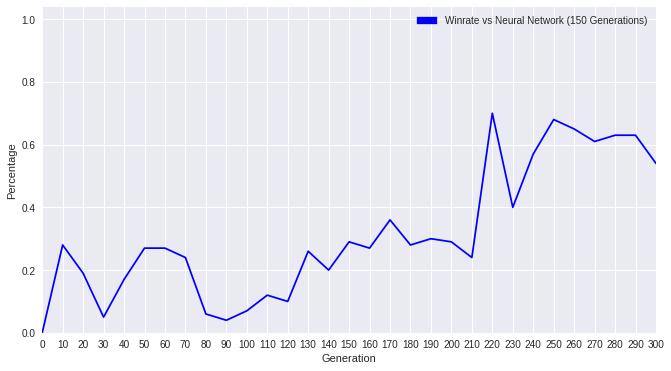
\includegraphics[width=0.7\textwidth]{graphics/winratevsneuralnetwork.png}
        \end{center}
        \caption{Winrate vs neural network trained for 150 generations}
        \label{fig:winratevsneuralnetwork}
    \end{small}
\end{figure}

Examining the neural network is only interesting if the neural network can effectively play the game. We first examine the history neural network playing against an agent that only takes random moves, on every $10$ generations. The win rate over generations can be seen in Figure \ref{fig:winratevsrandom}. It is clear that very early on in the training process, almost immediately after generation $10$ our agent performs nearly perfectly against the random agent. This implies that the agent does indeed learn some strategy in the game. The next agent we tried the neural network against, was an agent that does regular Monte-Carlo tree search on the game space with $100$ iterations of rollout for each move. A graph showing the win rate over generations is depicted in Figure \ref{fig:winratevsmcts}. Again, our agent quickly learns some strategy and can win often, although doesn't achieve a perfect win rate after $300$ generations. The last agent we tested against was the neural network itself, although only trained to $150$ generations. The graph in Figure \ref{fig:winratevsneuralnetwork} shows win rate. As expected the agent performs poorly until it has trained for more than $150$ generations.

These results imply that our agent certainly understands how to play the game of breakthrough to a certain level. However, an intermediate level human player would most often be able to win the agent, based on the author's experience playing against it. Note, that the main focus of this was not to create an expert level agent. Rather to, gauge into the concepts the agent learns as described in the next section.

\section{Evaluating the improvements of the Neural Network over generations}

To test which HLC the neural network places its emphasis on during training we trained a neural network for $300$ generations, taking snapshots of the network every $10$ generations. We then had the neural network play against itself for $100$ games, collecting the states it encountered during play. These states were then examined by a concept activation vector representing these HLCs.

We test four concepts \textit{Material Advantage}, \textit{Aggressiveness}, \textit{Unity}, and \textit{Lorentz-Horey}.

\subsection{Description of concepts}

\begin{figure}
    \begin{small}
        \begin{center}
            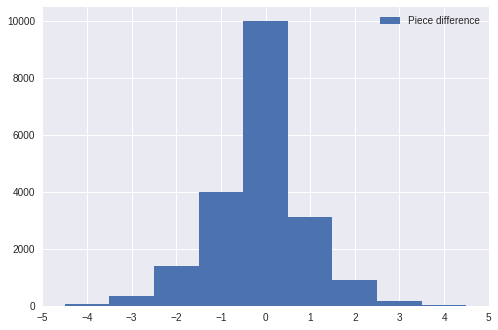
\includegraphics[width=0.95\textwidth]{graphics/dist_number_adv}
        \end{center}
    \end{small}
    \caption{Distribution of piece amount difference}
    \label{fig:distnumberadv}
\end{figure}

The first concept we examine is Material Advantage which conveys the idea of having more pawns than your opponent. When faced with a board it is difficult to argue for whether having a single pawn up on your opponent constitues as Material Advantage or three. In order to an appropriate value for this case we used the neural network that had been trained for $300$ generations to generate $20000$ unique states. The distribution of these states' difference of pawns can be seen in Figure \ref{fig:distnumberadv}. From examining the distribution and examining samples we selected the breakpoint of $\geq 2$, meaning that if you have $2$ pieces on your opponent you are in a state that has this concept. From the $20000$ states only $5.5\%$ of states have this concept.

\begin{figure}
    \begin{small}
        \begin{center}
            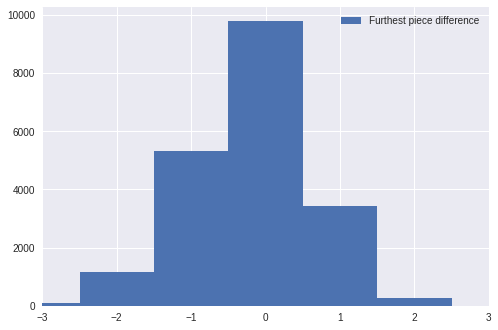
\includegraphics[width=0.95\textwidth]{graphics/dist_aggressiveness}
        \end{center}
        \caption{Distribution of difference of furthest pawns}
        \label{fig:distaggressiveness}
    \end{small}
\end{figure}

The next concept is Aggressiveness, which describes how much closer your furthest piece is to the opponents edge than your opponents furthest piece to your edge. This is then the minimum amount of how many moves it will take you to win the game. A distribution of these values can be seen in Figure \ref{fig:distaggressiveness}. We examined the distribution, and sampled states from various breaking points and decided on the value of $\geq 1$. That is if the value of a state's furthest piece difference is greater than or equal to $1$ that state has the concept of Aggressiveness. From the dataset $18.3\%$ of states have this concept.

\begin{figure}
    \begin{small}
        \begin{center}
            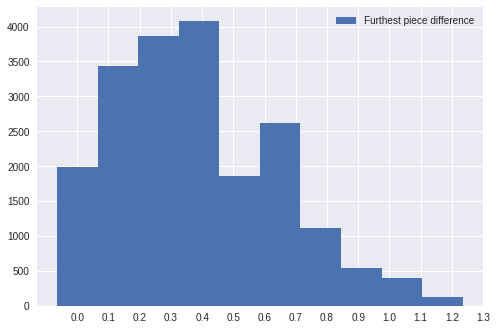
\includegraphics[width=0.95\textwidth]{graphics/dist_unity}
        \end{center}
        \caption{Difference of distance from center}
        \label{fig:distunity}
    \end{small}
\end{figure}

Our third concept is Unity. This concept represents the absolute average distance of your pawns from the center row of your pawns, and is calculated as follows: the row of your furthest pawn from the starting row $r_{far}$, the row of your nearest pawn from the starting row $r_{near}$. Finding the middle row is then $\frac{r_{far} + r_{near}}{2}$, we then take the absolute of the average distance from all of the players pawns to that row. The distribution of the average distance values is shown in Figure \ref{fig:distunity}. From sampling states from several points we decided on a breakpoint of $\le 0.25$ for identifying states as states where the Unity concept is precent. The value of $0.25$ generally allows your states to have two rows that have the majority of the pawns and one or two pawns one row away from the group. From the dataset of 20,000 states $20\%$ of states have this concept.

\begin{figure}
    \begin{small}
        \begin{center}
            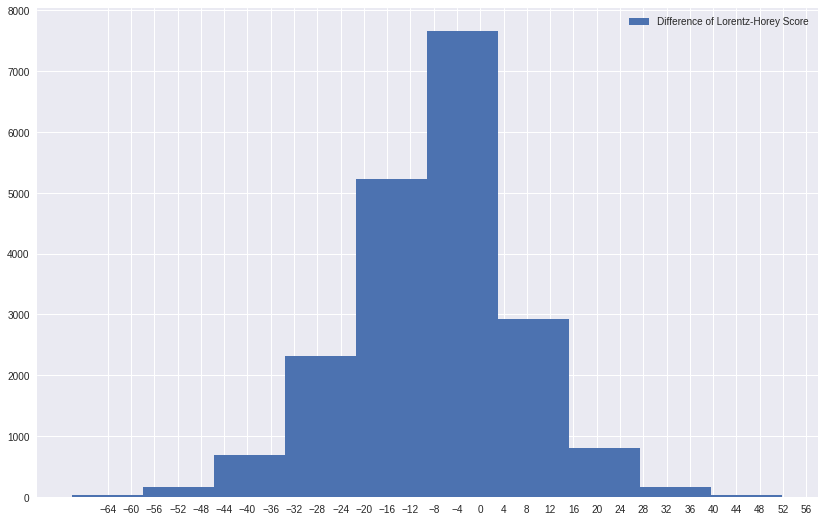
\includegraphics[width=0.95\textwidth]{graphics/dist_lorentz}
        \end{center}
        \caption{Difference of Lorentz-Horey Score}
        \label{fig:distlorentz}
    \end{small}
\end{figure}

\begin{table}[]
    \centering
    \begin{tabular}{|c|c|c|c|c|c|}
        \hline
        5  & 15 & 5  & 5  & 15 & 5  \\\hline
        2  & 3  & 3  & 3  & 3  & 2  \\\hline
        4  & 6  & 6  & 6  & 6  & 4  \\\hline
        7  & 10 & 10 & 10 & 10 & 7  \\\hline
        11 & 15 & 15 & 15 & 15 & 11 \\\hline
        21 & 21 & 21 & 21 & 21 & 21 \\\hline
    \end{tabular}
    \caption{Lorentz-Horey cell values, from white players point of view}
    \label{table:lorentzcell}
\end{table}

The last concept we examined was the Lorentz-Horey. This concept is a popular heuristic in Breakthrough defined in the paper by Lorentz \& Horey \cite{lorentz:heuristic}. For this heuristic, we give each cell on the board a point value. For a given player the heuristic is then the sum of the cell values where they have pawns. The cell values are shown in Table \ref{table:lorentzcell}. The matrix shown is flipped from the black player's point of view. The values are selected in such a way that as your pawn approach the opponent's side their value increases, having pieces on the edge isn't optimal, as such a pawn will only be able to capture in one direction and can not escape capture as easily. To select the breakpoint for Lorentz-Horey heuristic, we generate a distribution of the difference in Lorentz-Horey Score over our dataset. The resulting distribution is shown in Figure \ref{fig:distlorentz}. Our examination lead us to select the value of $5$, as a breakpoint indicating that a state has the concept of Lorentz-Horey. Out of our dataset of 20,000 states $29.4\%$ of states have this concept.

\subsection{Material Advantage}

\begin{figure}[]
    \centering
    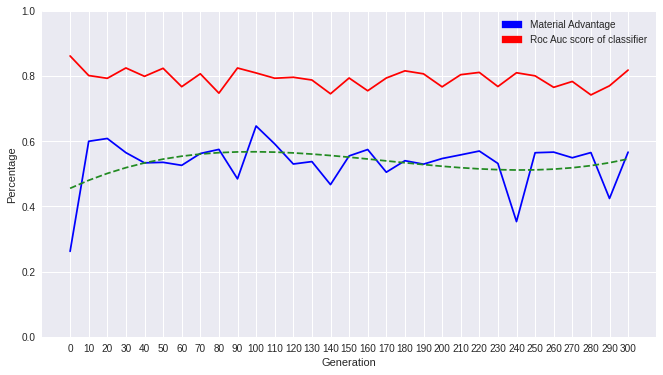
\includegraphics[width=0.7\textwidth]{graphics/number_pawns_trend}
    \caption{Percentage of selected states containing the HLC Material Advantage}
    \label{fig:numberadvantage}
\end{figure}

The Figure \ref{fig:numberadvantage}. shows that throughout training the Material Advantage HLC is only ever a slight factor in the selection of states and we can say that the neural network doesn't consider number advantage in its selection process.

\subsection{Agressiveness}

\begin{figure}[]
    \centering
    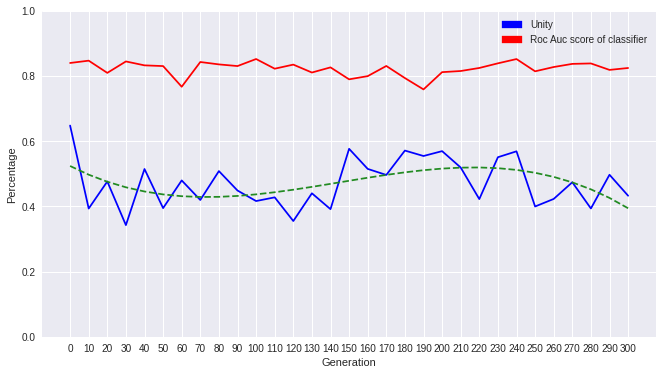
\includegraphics[width=0.7\textwidth]{graphics/most_advanced_trend.png}
    \caption{Percentage of selected states containing the HLC aggressiveness}
    \label{fig:aggressiveness}
\end{figure}

From Figure \ref{fig:aggressiveness}. we can see that the aggressiveness HLC is a growing factor over as the neural network is trained. As a piece can always move forward, if your opponent does not capture that piece, this concept relates to how many moves it will take for you to win. Generally, when your opponent is not playing well this concept does well, and quickly becomes a bad heuristic in classical search algorithms.

\subsection{Unity}

\begin{figure}[]
    \centering
    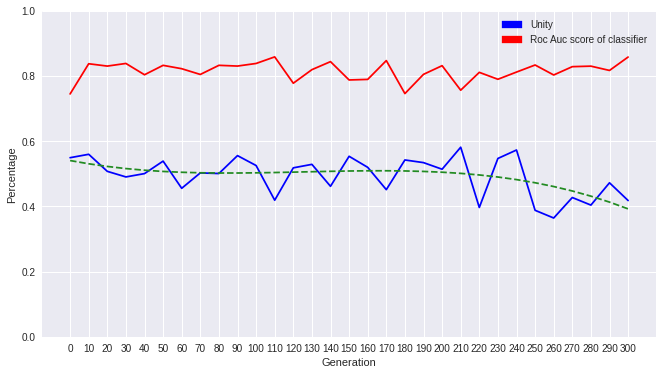
\includegraphics[width=0.7\textwidth]{graphics/unity_trend.png}
    \caption{Percentage of selected states containing the HLC unity}
    \label{fig:unity}
\end{figure}

\begin{figure}
    \begin{small}
        \begin{center}
            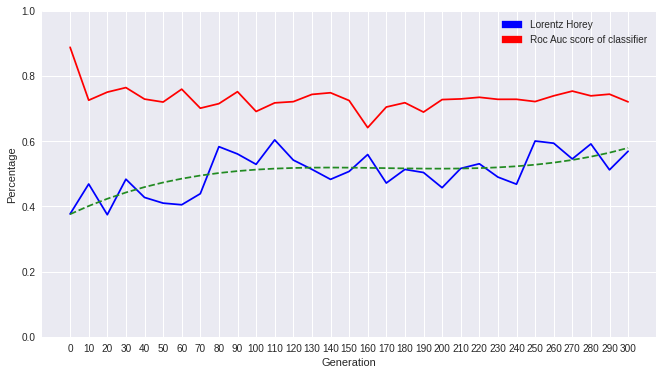
\includegraphics[width=0.95\textwidth]{graphics/lorentz_horey_trend.png}
        \end{center}
        \caption{Percentage of selected states containing the HLC Lorentz-Horey}
        \label{fig:lorentzheuristic}
    \end{small}
\end{figure}

The literature of Breakthrough implies that being patient and waiting until your opponent makes a mistake is generally the preferred strategy for winning.\cite{lorentz:heuristic} Examining Figure \ref{fig:lorentzheuristic}, we can see that the trend of using this HLC increases over time. As this heuristic is the one most often cited as a successful strategy in Breakthrough, it is interesting to see that our Breakthrough agent is gradually learning a similar concept.

\section{Summary}

In this section we discussed some concepts that we believed would be representative of concepts that a nerual network would learn over time playing Breakthrough. An important note is that there are an infinite amount of concepts, and there could exist some that the neural network uses extensively that we overlooked. We examined the neural network against these concepts. In the following chapter we will discuss the next steps for this research.